\cotefile{109}
\scanpage{31}
% One handwritten correction list. Two vertical traces are preserved geometrically;
% their ink/material origin is unassigned. Circular edge impressions are material.
\noindent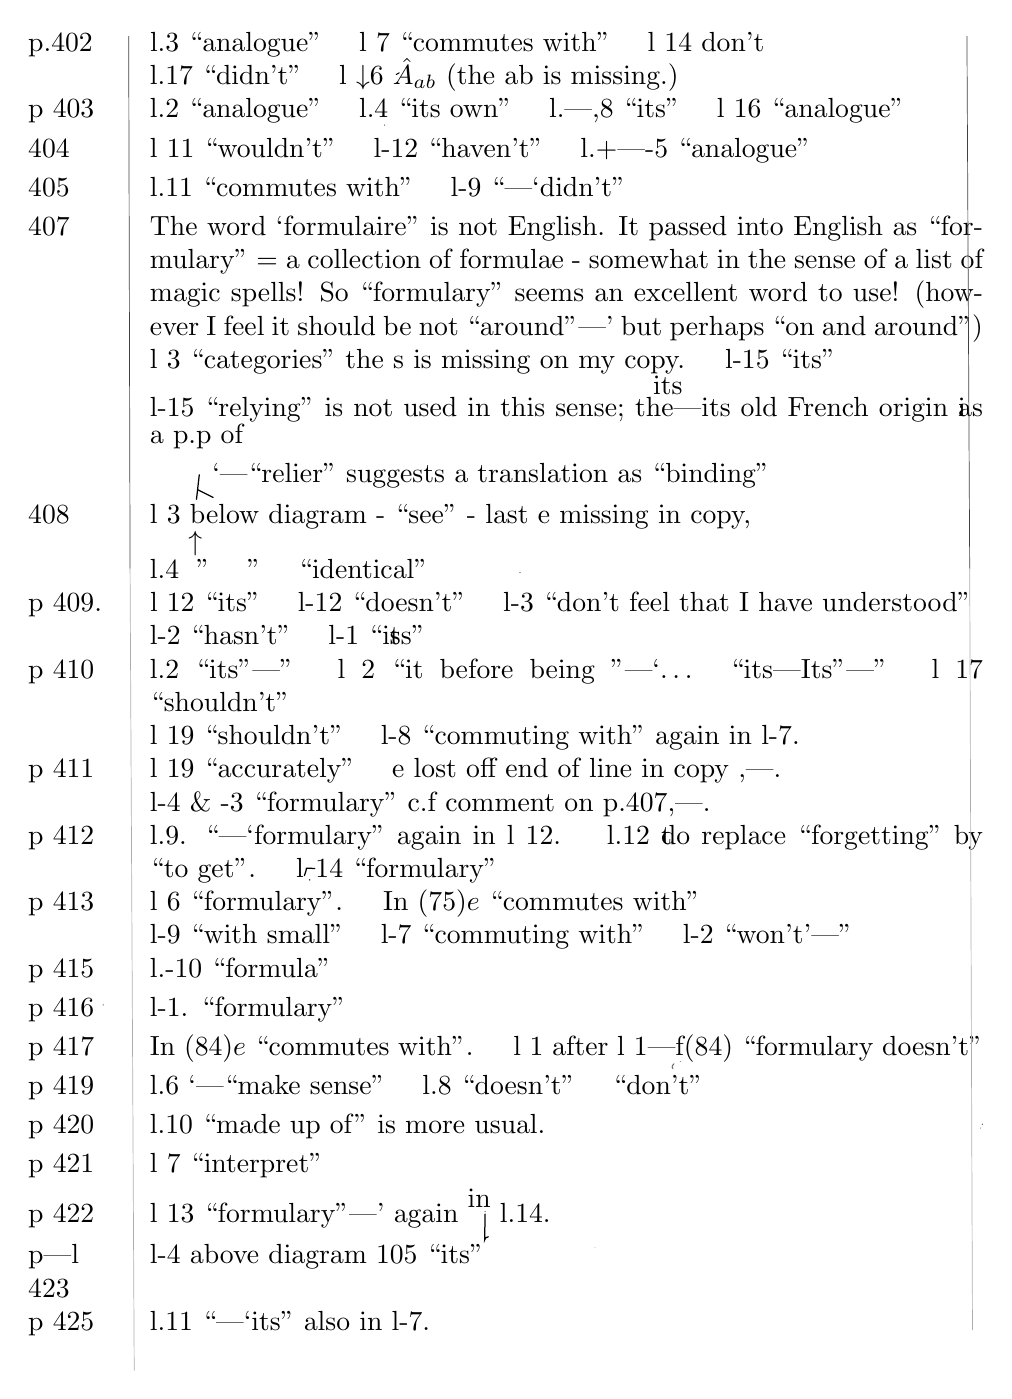
\begin{tikzpicture}
\node[anchor=north west,inner sep=0pt] (sheet031B) {%
\begin{minipage}{\linewidth}
\begin{tabular}{@{}p{3.4em}@{\hspace{1em}}p{\dimexpr\linewidth-4.4em\relax}@{}}
p.402 & l.3 ``analogue'' \quad l 7 ``commutes with'' \quad l 14 don't\par l.17 ``didn't'' \quad l $\downarrow$6 \tikz[baseline=(hat031.base)]{\node[inner sep=0pt] (hat031) {$\hat{A}_{ab}$};\draw[overlay,line width=.35pt,line cap=round] ([xshift=.14em,yshift=.85ex]hat031.base west)--([xshift=.25em,yshift=1.0ex]hat031.base west);} (the ab is missing.) \\[.5ex]

p 403 & l.2 ``analogue'' \quad \tikz[baseline=(ref403B.base)]{\node[inner sep=0pt] (ref403B) {l.4};\fill ([xshift=-.15em,yshift=-.6ex]ref403B.base east) circle (.045ex);} ``its \deleted{own}'' \quad l\unsure{.|,}8 ``its'' \quad l 16 ``analogue'' \\[.5ex]

404 & l 11 ``wouldn't'' \quad l-12 ``haven't'' \quad l.\unsure{+|-}5 ``analogue'' \\[.5ex]

405 & l.11 ``commutes with'' \quad l-9 \unsure{``|`}didn't'' \\[.5ex]

407 & The word `formulaire'' is not English. It passed into English as ``formulary'' $=$ a collection of formulae - somewhat in the sense of a list of magic spells! So ``formulary'' seems an excellent word to use! (however I feel it should be not ``around\unsure{''|'} but perhaps ``on and around'')\par l 3 ``categorie\uline{s}'' the s is missing on my copy. \quad l-15 ``its''\par l-15 ``relying'' is not used in this sense; \tikz[baseline=(old407B.base)]{\node[inner sep=0pt] (old407B) {\deleted{\unsure{the|its}}};\node[anchor=south west,inner sep=0pt] at ([xshift=.65em,yshift=.1ex]old407B.north west) {\inserted{its}};} old French origin \tikz[baseline=(as407B.base)]{\node[inner sep=0pt] (as407B) {\deleted{\unsure{i}}};\node[anchor=base west,inner sep=0pt] at (as407B.base west) {a};}s \tikz[baseline=(rel407C.base)]{\node[inner sep=0pt] (rel407C) {\unsure{`|``}relier''};\node[anchor=south,inner sep=0pt] at ([xshift=-.55em,yshift=1.1ex]rel407C.north west) {\inserted{a p.p of}};\draw[line width=.45pt,line cap=round] ([xshift=-.45em,yshift=.65ex]rel407C.base west)--([xshift=-.55em,yshift=-1.4ex]rel407C.base west);\draw[line width=.45pt,line cap=round] ([xshift=-.51em,yshift=-.6ex]rel407C.base west)--([xshift=.05em,yshift=-1.25ex]rel407C.base west);} suggests a translation as ``binding'' \\[.5ex]

408 & l 3 below diagram - ``see'' - last e missing in copy,\par l.4 \tikz[baseline=(ditto408B.base)]{\node[inner sep=0pt] (ditto408B) {''};\node[anchor=south,inner sep=0pt] at ([xshift=-.3em,yshift=.2ex]ditto408B.north) {$\uparrow$};} \quad '' \quad \tikz[baseline=(identical408B.base)]{\node[inner sep=0pt] (identical408B) {``identical''};\fill ([xshift=3.3em,yshift=.5ex]identical408B.base east) circle (.045ex);} \\[.5ex]

p 409. & l 12 ``its'' \quad l-12 ``doesn't'' \quad l-3 ``don't feel that I have understood''\par l-2 ``hasn't'' \quad l-1 ``i\tikz[baseline=(old409B.base)]{\node[inner sep=0pt] (old409B) {\deleted{\unsure{s}}};\node[anchor=base west,inner sep=0pt] at (old409B.base west) {t};}s'' \\[.5ex]

p 410 & \deleted{l.\unsure{2}} ``\deleted{its}\unsure{\deleted{''}|''} \quad l 2 ``it \uline{before} being \unsure{''|`}\ldots{} ``\deleted{\unsure{its|Its}}\unsure{\deleted{''}|''} \quad l 17 ``shouldn't''\par l 19 ``shouldn't'' \quad l-8 ``commuting with'' again in l-7. \\[.5ex]

p 411 & l 19 ``accurately'' \quad e lost off end of line in copy \unsure{,|.}\par l-4 \& -3 ``formulary'' c.f comment on p.407\unsure{,|.} \\[.5ex]

p 412 & l.9. \unsure{``|`}formulary'' again in l 12. \quad l.12 \tikz[baseline=(old412B.base)]{\node[inner sep=0pt] (old412B) {\deleted{\unsure{t}}};\node[anchor=base west,inner sep=0pt] at (old412B.base west) {d};}o replace ``forgetting'' by ``to get''. \quad l\tikz[baseline=0pt,x=1ex,y=1ex]{\draw[line width=.45pt,line cap=round] (.12,.15)..controls(.27,.4)and(.24,.65)..(.3,.78)--(1.0,.75);\fill (.57,-.2) circle (.065);}14 ``formulary'' \\[.5ex]

p 413 & l 6 ``formulary''. \quad In $(75)e$ ``commutes with''\par l-9 ``with small'' \quad l-7 ``commuting with'' \quad l-2 ``won't\unsure{'|''} \\[.5ex]

p 415 & l.-10 ``formula'' \\[.5ex]

\tikz[baseline=(page416B.base)]{\node[inner sep=0pt] (page416B) {p 416};\fill ([xshift=.3em,yshift=.95ex]page416B.base east) circle (.045ex);} & l-1. ``formulary'' \\[.5ex]

p 417 & In $(84)e$ ``commutes with''. \quad l 1 after \tikz[baseline=(old417.base)]{\node[inner sep=0pt] (old417) {\deleted{\unsure{l 1|f}}};\fill[overlay,black!75] ([xshift=-.15em,yshift=-.5ex]old417.base east) circle (.04ex);\draw[overlay,black!60,line width=.35pt,line cap=round] ([xshift=-.38em,yshift=-.7ex]old417.base east)..controls([xshift=-.47em,yshift=-.9ex]old417.base east)and([xshift=-.46em,yshift=-1.05ex]old417.base east)..([xshift=-.42em,yshift=-1.12ex]old417.base east);}(84) ``formulary doesn't'' \\[.5ex]

p 419 & l.6 \unsure{`|``}make sense'' \quad l.8 ``doesn't'' \quad ``don't'' \\[.5ex]

p 420 & l.10 ``made up of'' is more usual. \hfill\tikz[baseline=0pt,x=1ex,y=1ex]{\fill (.12,.8) circle (.045);\fill (-.03,.48) circle (.035);} \\[.5ex]

p 421 & l 7 ``interpret'' \\[.5ex]

p 422 & l 13 ``formulary\unsure{''|'} again \tikz[baseline=0pt,x=1ex,y=1ex]{\path (0,0)--(.9,0);\node[anchor=south,inner sep=0pt] at (.1,1.2) {\inserted{in}};\draw[line width=.45pt,line cap=round] (.6,.68)--(.56,-1.5)..controls(.57,-1.35)and(.7,-1.22)..(.87,-1.23);\fill (.6,.88) circle (.045);} l.14. \\[.5ex]

\unsure{p|l} 423 & l-4 above diagram 105 \tikz[baseline=(its423B.base)]{\node[inner sep=0pt] (its423B) {``its''};\fill[black!55] ([xshift=4em,yshift=1.35ex]its423B.base east) circle (.035ex);} \\[.5ex]

p 425 & l.11 \unsure{``|`}its'' also in l-7. \\[.5ex]

\end{tabular}
\end{minipage}};
% BEGIN left-vertical-trace
\path (sheet031B.north west) -- (sheet031B.south west) coordinate[pos=.41] (trace031Bleftmid);
\draw[black!75,line width=.25pt] ([xshift=3.65em,yshift=-.7ex]sheet031B.north west) -- ([xshift=3.7em]trace031Bleftmid);
\draw[black!32,line width=.25pt] ([xshift=3.7em]trace031Bleftmid) -- ([xshift=3.85em,yshift=-2ex]sheet031B.south west);
% END left-vertical-trace
% BEGIN right-vertical-trace
\path (sheet031B.north east) -- (sheet031B.south east) coordinate[pos=.41] (trace031Brightmid);
\draw[black!75,line width=.25pt] ([xshift=-.6em,yshift=-.7ex]sheet031B.north east) -- ([xshift=-.5em]trace031Brightmid);
\draw[black!32,line width=.25pt] ([xshift=-.5em]trace031Brightmid) -- ([xshift=-.4em,yshift=1.4ex]sheet031B.south east);
% END right-vertical-trace
\end{tikzpicture}
% archive sheet number: 30
